\documentclass{article}
\usepackage{graphicx}
\usepackage{algorithm}
\usepackage[noend]{algorithmic}
\usepackage{subfigure}
\usepackage{amssymb, amsmath, graphicx, charter, latexsym}
\usepackage{layouts}
\usepackage[letterpaper]{geometry}
\usepackage{enumerate}
\usepackage{epstopdf}
\usepackage{ragged2e}
%\usepackage{times}
\usepackage{mathtools}
%\usepackage[scaled]{helvet}
\usepackage{mathptmx}
\usepackage{verbatim}
\usepackage{listings}
\usepackage{siunitx}

\lstset{
basicstyle=\ttfamily,
}

\begin{document}

\title{ECEN 689: Real-Time Wireless Networks\\ Project 1, due on 2/26}
\date{}
\author{%
Ping-Chun Hsieh\\
UIN: XXXXXXXXXX\\
\texttt{lleyfede@tamu.edu}
\and
Tao Zhao\\
UIN: 825000452\\
\texttt{alick@tamu.edu}
\and
Dongni Han\\
UIN: XXXXXXXXXX\\
\texttt{handongni2015@tamu.edu}
}
\maketitle

\section*{Terminology}

In our report, we use ``server'' to denote the WiFi access point (AP), and
``client'' to denote the terminal device such as a mobile phone, a tablet, and
so on. Throughout our simulation, we let node $0$ be the server, and node $1$ be
the client, which correspond to the device A and B in the problem descriptions
respectively.

S-WiFi is the name of our application as well as our project. It stands for
Smart WiFi, or whatever you think it is.

\section{Downlink Transmissions}

\section{Uplink Transmissions with PCF}
In uplink transmissions with PCF, the server sends out a POLL packet to
the client periodically. When the client receives the POLL packet, and has data
to be transmitted, it replies with a data packet.

Since ns-2 does not have a PCF module, we mimic the PCF behavior in the
application layer. Specifically, we define a new packet type
\lstinline|SWiFi_PKT_POLL|, and a new command ``poll'' for the S-WiFi
application. We let node 0 call the poll command every \SI{10}{ms}.
During the execution of the poll command, we create a new packet, set the packet
type \lstinline|SWiFi_PKT_POLL| and record the current time as the send time in
the packet header, and then send it out.

When the client receives a packet and finds its packet type is
\lstinline|SWiFi_PKT_POLL|, it acquires the send time, creates a new packet of
type 2 (data packet from client to server), and carries the old send time in its
header. Then it sets the packet size, fills the payload with its data message
(a predefined string in our simulation), and sends it out.

When the server receives a packet and finds it is a data packet from client to
server, it decodes the data message and gets the old send time $T_\text{s}$ from
the packet header. Let $T$ denote the current reception time. The
round-trip-time (RTT) is calculated by:
\begin{equation}
	\text{RTT} = T - T_s
\end{equation}
Afterwards, the client calls a Tcl instproc (member function of a class
in Tcl's terminology) \lstinline|recv| with the data message and RTT as the
arguments. \lstinline|recv| simply stores the information into a log file.

\section{Transmission Reliability}

\begin{figure*}[h]
\centering
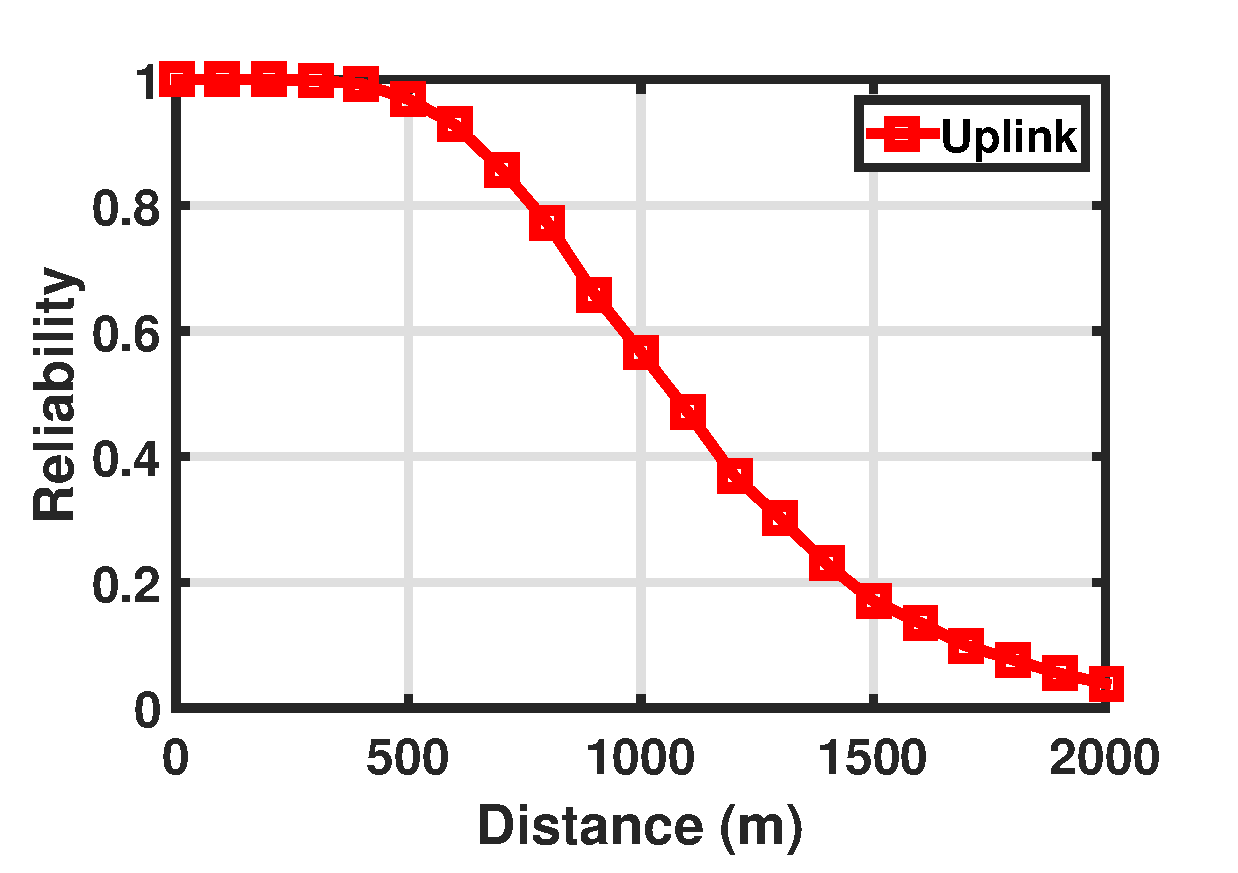
\includegraphics[width=3.5in]{p3_uplink.eps}
\caption{Reliability versus distance for uplink transmissions.}
\end{figure*}

\section{Measuring Delays}
\section{Preferences for Final Report}
We prefer topic 2 to topic 3, and prefer topic 3 to topic 1. ($2 \succ 3 \succ 1$)


\end{document}
